\section{Implementation details}
\label{app:implementation}

\paragraph*{C2 local actions.}
For each selected chart, split proposes a cut along the dominant curvature direction estimated from per-face normals and the chart covariance frame. Merge-with-neighbor evaluates adjacent charts in nearest-neighbor order by seam residual and keeps the merge with the lowest C2 score. Boundary slide moves boundary texels for \(N\) small steps along the gradient flow of the face residual \(e_f\), clamped by the distortion guard. Local ARAP keeps the chart center anchored and runs 10 local/global iterations before repacking the chart under the fixed atlas-size budget.

\paragraph*{Beam scoring and residual attribution.}
Candidates are scored in the order split, merge, boundary slide, and local ARAP for each selected chart, then pruned to beam size 4. The render term in \cref{eq:c2_cost} is measured as
\begin{equation}
\Delta\mathcal{L}_{render}(c,a)=
\mathcal{L}_{render}(U_{c,a})-\mathcal{L}_{render}(U_0),
\end{equation}
on the proposal split $\Vprop \times \Lprop$ only; this split is disjoint from the gate split $\Vgate \times \Lgate$ used by C5 and from the test split $\Vtest \times \Ltest$ used to report headline metrics (\cref{sec:exp_setup,tab:a1_split}). Residual attribution uses the nvdiffrast face-id buffer: per-pixel proposal-split RGB residuals are scattered with \(\mathrm{scatter\_add}\) into a per-face accumulator and normalized by the visible sample count before chart aggregation.

\paragraph*{Runtime and memory.}
\begin{table}[t]
\centering
\scriptsize
\caption{End-to-end wall-clock and peak GPU memory for representative cases on a single RTX 4090 (PyTorch 2.7.1 cu128, bf16 baker). Wall-clock includes oracle PBR setup, baking, residual attribution, candidate search, C5 audit, and final atlas export; PartUV preprocessing of the upstream atlas is excluded and reported separately.}
\label{tab:runtime}
\begin{tabular}{@{}lrrrl@{}}
\toprule
Case & Faces & Wall-clock (s) & Peak GPU (GB) & C5 \\
\midrule
spot / PartUV (accept) & 372 & 1313 & 0.59 & accept \\
bunny / PartUV (accept) & 1280 & 1814 & 0.59 & accept \\
spot / xatlas (rollback) & 372 & 2578 & 0.53 & rollback \\
objaverse / xatlas (rollback) & 192 & 166 & 0.53 & rollback \\
proc\_warped\_cylinder / PartUV (accept) & 1152 & 158 & 0.58 & accept \\
ts\_animal / PartUV (real, accept) & 3068 & 2777 & 0.59 & accept \\
f3d\_animal / PartUV (real, accept) & 3068 & 16772 & 0.96 & accept \\
\bottomrule
\end{tabular}
\end{table}

\Cref{tab:runtime} reports end-to-end wall-clock and peak GPU memory on a single RTX 4090. Procedural and small-asset cases finish in 2--5 minutes; larger meshes (bunny, ts\_animal, f3d\_animal) need 30~min--5~h dominated by C2 candidate search rather than rendering. Peak GPU memory stays under 1~GB for all listed cases. PartUV upstream preprocessing is independent and is the practical bottleneck for the 18 deferred real meshes (\cref{sec:limitations}); the differentiable baker, residual attribution, C2 search, and C5 audit themselves do not require multi-GPU.

\paragraph*{Renderer and C5 thresholds.}
The renderer uses nvdiffrast \(\mathrm{rasterize\_cuda}\) for visibility, a custom GGX shader for albedo/normal/roughness/metallic relighting, fp16 texture and shading buffers, and fp32 reductions for metrics. The logged C5 gate uses \(\delta_p=0.3\) dB, \(\delta_s=8\%\) relative seam drop, \(\epsilon_D=3.0\) for maximum distortion \(Q_{95}\), and \(\Delta_C=\pm10\%\) chart-count tolerance.

\section{Baseline reproduction failure table}
\label{app:baseline_failure}

\begin{table*}[t]
\centering
\scriptsize
\caption{Baseline reproduction scope. Only real integrated baselines are used for main numerical comparisons; partial or failed baselines are reported to bound the claims.}
\label{tab:baseline_failure}
\begin{tabularx}{\linewidth}{@{}l l l X@{}}
\toprule
Baseline & Status & Used in main table & Reproduction note \\
\midrule
xatlas & real & yes & Python xatlas integration ran on all three main assets and passed the matched protocol. \\
Blender Smart UV & real & yes & Blender 3.0.1 Smart UV ran after wrapper fixes; it is a useful production baseline but often violates chart-count or utilization matching because it follows a different atlas paradigm. \\
PartUV & real & yes & Real subprocess integration produced part-aware atlases for spot, bunny, and Objaverse; PartUV is the primary weak-baseline case where residual repair triggers. \\
matched oracle & real control & yes & Self-implemented oracle UV reference used as an upper-bound control; infinite PSNR rows are rolled back because there is no residual-backed improvement to deploy. \\
FlexPara & partial & no & Repository constraints required Python 3.9, PyTorch 1.10/CUDA 11.1 compatibility, custom CUDA ops, and unavailable shipped checkpoints; only a proxy was available, so it is excluded from main claims. \\
OT-UVGS & adjacent/proxy & no & Treated as a capacity-allocation reference rather than a verified mesh-UV baseline; no full direct mesh reproduction is claimed. \\
Flatten Anything & failed & no & Environment and checkpoint requirements could not be verified in the available run budget. \\
ParaPoint & failed & no & Repository or checkpoint availability was not verified, so no numerical comparison is claimed. \\
visibility-param control & proxy & no & Included as an explicit attempt at the review guardrail baseline, but no public implementation was available for a real reproduction. \\
\bottomrule
\end{tabularx}
\end{table*}

\section{Additional qualitative result}
\label{app:additional_qual}

\begin{figure*}[t]
  \centering
  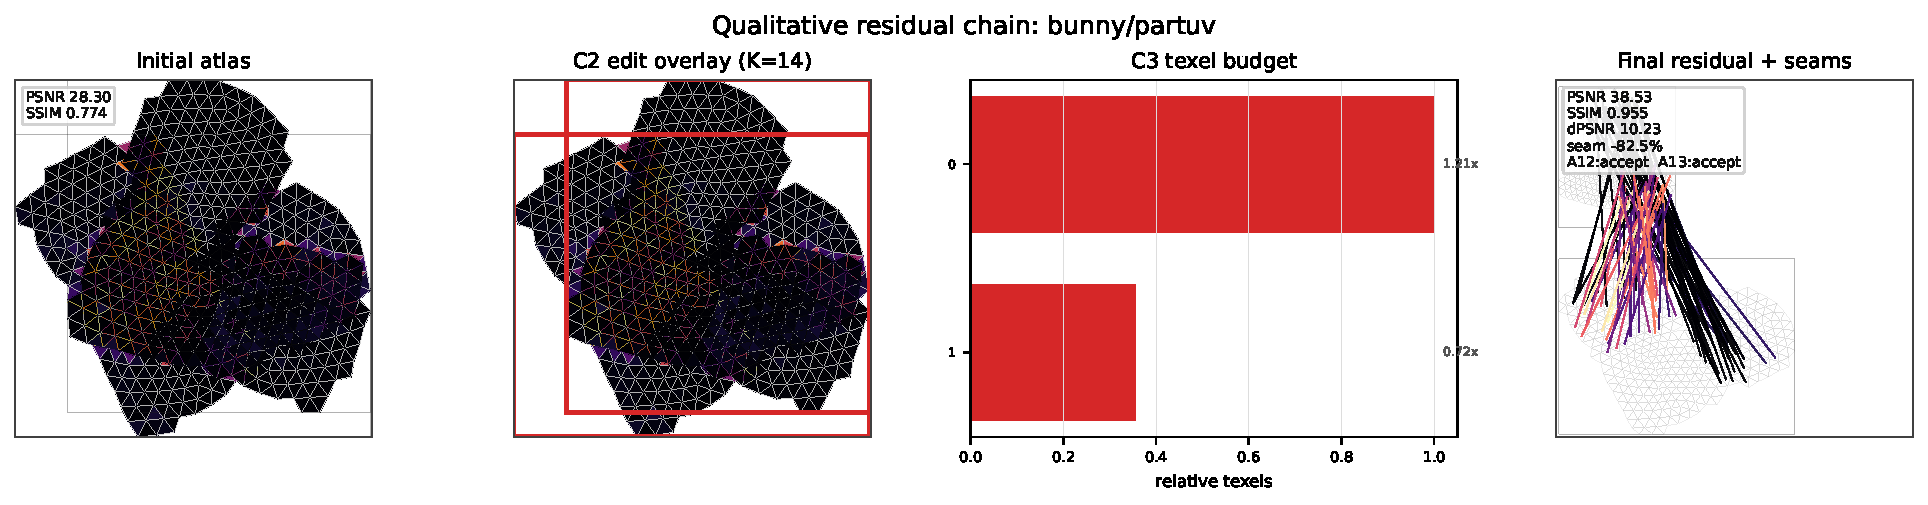
\includegraphics[width=0.88\linewidth]{figures/qualitative_residual_chain/bunny_partuv_residual_chain.pdf}
  \caption{Bunny/PartUV residual chain. The same residual-driven pipeline accepts the local repair and improves relit \PSNR{} from 28.30 dB to 38.53 dB.}
  \label{fig:bunny_chain}
\end{figure*}

\Cref{fig:bunny_chain} complements the spot hero case in \cref{fig:spot_chain}. The bunny atlas has fewer charts, so the edited-chart ratio is high even though the absolute edit count is small. This is why the paper reports edited counts and not only edited percentages.
